\documentclass{standalone}
\usepackage{tikz}
\usetikzlibrary{intersections,shapes.arrows}

\newcommand\Dist[1]{\phantom{\rule{#1}{4pt}}}

\begin{document}

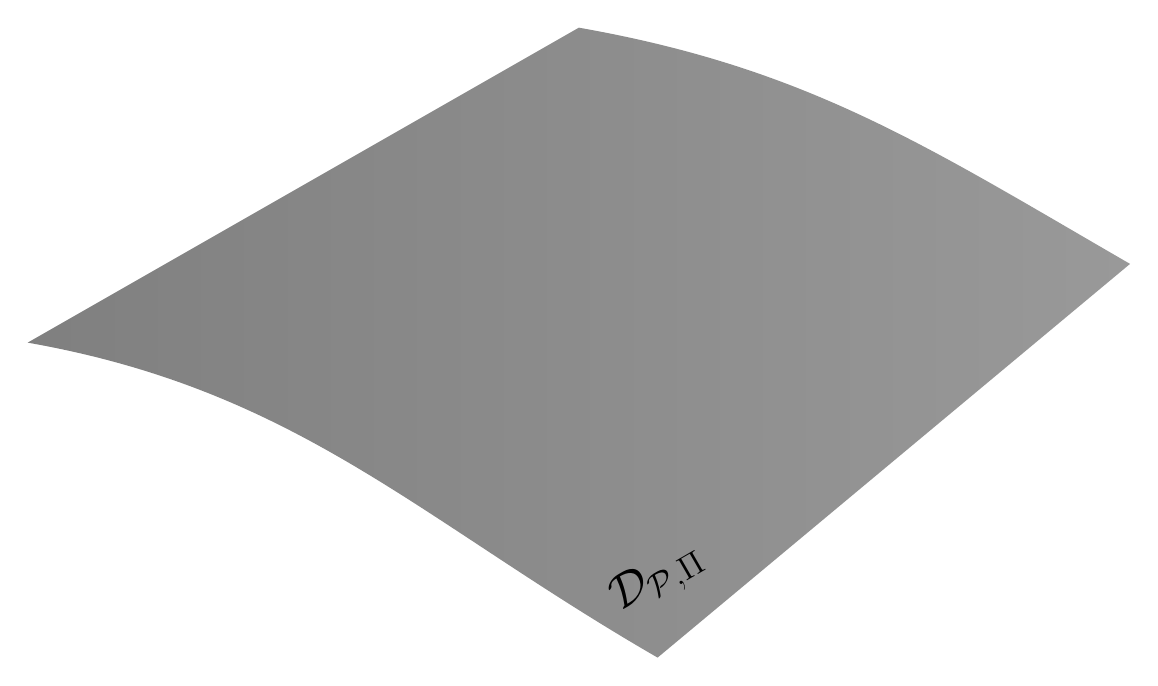
\begin{tikzpicture}
% we draw the surface
\shade[left color=black!50,right color=gray!80] 
  (0,0) to[out=-10,in=150] (8,-4) -- (14,1) to[out=150,in=-10]
  (7,4) -- cycle;
  
  % p hat
  %\draw[fill] (4,4) circle (3pt);
  
  %\shade[ball color = orange!90!black, opacity = 0.6] (4,0) circle (4cm);

 % \draw[dashed] (4,0) -- node[above]{$\epsilon$} (0,0);
  
  % p
%  \draw[fill, color=red] (7,2) circle (3pt);
%  
%  % q
%  \draw[fill, color=red] (4,0) circle (3pt);
%  
%  \draw[name path=pq, dashed] (4.1,0) to[out=-10,in=150] (6.9,2.1);
%
%  \draw[name path=phatq, dashed] (7,2.1) to (4,4);
%  
%  \draw[name path=phatp, dashed] (4,0.1) to (4,4);
  
  
%  we place the label phat
%\node (phat) [font=\sffamily] at (4,4.4) {\LARGE $d$};
%%  we place the label p
%\node (q) [font=\sffamily] at (7.4,2.2) {\LARGE $\widehat{d}$};
%%  we place the label q
%\node (p) [font=\sffamily] at (3.5,0.2) {\LARGE $d^{P,\pi}$};
%
%% we add some labels
%\node[font=\sffamily] at (6,0.4) {\large $D_{KL}(\widehat{d} \| d^{P,\pi})$};
%
%% we add some labels
%\node[font=\sffamily] at (3.8,2) {\Large $\epsilon$};
%% we add some labels
%\node[font=\sffamily] at (6.2,3) {\Large $\leq \epsilon$};

% we add some labels
\node[rotate=30] at (8, -3) {\LARGE $\mathcal{D}_{\mathcal{P} , \Pi}$};

\end{tikzpicture}
\end{document}